\documentclass[a4paper,titlepage]{book}
\usepackage{frontespizio}
\usepackage[italian]{babel}
\usepackage[utf8]{inputenc}
\usepackage[linktocpage=true]{hyperref}

\usepackage{usecases}

\usepackage{tikz}
\usetikzlibrary{arrows,shadows} % for pgf-umlsd
\usepackage[underline=true,rounded corners=false]{pgf-umlsd}

\usepackage{enumitem}
\setitemize{noitemsep,topsep=0pt,parsep=0pt,partopsep=0pt}

\usepackage[a4paper, total={6in, 9in}]{geometry}

\usepackage{listings}

\lstset{language=C, basicstyle=\small\ttfamily,
keywordstyle=\color{red}\bfseries,
commentstyle=\color{blue},
stringstyle=\color{magenta},
morecomment=[l][\color{magenta}]{\#},
numbers=left,
numberstyle=\tiny,
stepnumber=2,
frame=trBL,
emph={MODBUS_SERIAL_WAIT_FOR_RESPONSE,uart_rx_interrupt, FALSE, TRUE, MODBUS_GETDATA, MODBUS_GETADDY, MODBUS_GETFUNC, MODBUS_SERIAL_RX_BUFFER_SIZE, TIMEOUT, MODBUS_SERIAL_TIMEOUT},
emphstyle=\color{black}\bfseries,
morekeywords={int8_t, uint8_t, int16_t, uint16_t, function, exception, word, bool, BOOL, eMBParity, UCHAR, CHAR, ULONG, LONG, SHORT, USHORT, EMWIN_WIDGET_TYPE, WM_HWIN}
}



\begin{document}
\begin{frontespizio}
\Universita{Verona}
\Dipartimento{Informatica}
\Corso[Laurea]{Informatica}
\Titoletto{Tesi di laurea triennale}
\Titolo{Sistema domotico a basso costo\\pilotato con protocollo Modbus}
\Candidato[VR359169]{Enrico Giordano}
\Relatore{Prof. Graziano Pravadelli}
\Annoaccademico{2013-2014}
\end{frontespizio}




%%%%%%%%%%%%%%%%%%%%%%%%%%%%%%%%%%%%%%%%%%%%%%%%%%%%%%%%%%%%%%%%%%%%%%%%%%%%%%%%%%%%%%%%%%%%%%%%%%%%%%%%%%%%%%%%%%%%%%%%%%%%%%%%%%%%%%%%%
%%%%%%%%%%%%%%%%%%%%%%%%%%%%%%%%%%%%%%%%%%%%%%%%%%%%%%%%%%%%%%%%%%%%%%%%%%%%%%%%%%%%%%%%%%%%%%%%%%%%%%%%%%%%%%%%%%%%%%%%%%%%%%%%%%%%%%%%%
%%%%%%%%%%%%%%%%%%%%%%%%%%%%%%%%%%%%%%%%%%%%%%%%%%%%%%%%%%%%%%%%%%%%%%%%%%%%%%%%%%%%%%%%%%%%%%%%%%%%%%%%%%%%%%%%%%%%%%%%%%%%%%%%%%%%%%%%%
%%%%%%%%%%%%%%%%%%%%%%%%%%%%%%%%%%%%%%%%%%%%%%%%%%%%%%%%%%%%%%%%%%%%%%%%%%%%%%%%%%%%%%%%%%%%%%%%%%%%%%%%%%%%%%%%%%%%%%%%%%%%%%%%%%%%%%%%%

\chapter*{Introduzione}
La domotica è una scienza interdisciplinare che si occupa di creare oggetti utili a migliorare la qualità della vita nella casa e più in generale negli ambienti abitati, favorendo la serenità e facendo risparmiare tempo (e soprattutto denaro) per la gestione delle faccende domestiche.
 
Con l'avanzare della tecnologia, vengono utilizzati strumenti sempre più complessi, favorendo un sistema \textit{``user friendly''} ma costoso, che dal punto di vista finanziario non è accessibile per la maggior parte delle famiglie. Un fattore che avvicina gli sviluppatori a queste tecnologie è la semplicità di progettazione: più avanzata è l'architettura, quindi definibile \textit{``general purpoise''}, più è facile sviluppare nuovo software e mantenerlo nel tempo. Queste architetture però non sono dedicate esclusivamente all'ambito di utilizzo; questo è un fattore che impreziosisce tutto il progetto nel complesso e di conseguenza fa aumentare il prezzo di mercato del progetto stesso.

La soluzione a questo problema è progettare un sistema dedicato, \textit{``embedded''}, in grado di occuparsi esclusivamente di alcuni compiti e ottimizzato sia nei costi che nell'esecuzione delle operazioni specifiche. Questo può essere un limite per vari fattori, ossia difficoltà di sviluppo, difficoltà di scelta della componentistica, ottimizzazione di risorse e codice, però offre il vantaggio di essere un progetto a basso costo dal punto di vista sia hardware che software, in quanto si propone qualcosa di più semplice ma efficace.

~

Questo progetto rappresenta un piccolo sistema domotico con cui si controllano le luci di una casa e i vari sensori che monitorano le stanze, utilizzando un pannello di controllo Master che comunica con le diverse periferiche slave tramite protocollo Modbus.


\tableofcontents


%%%%%%%%%%%%%%%%%%%%%%%%%%%%%%%%%%%%%%%%%%%%%%%%%%%%%%%%%%%%%%%%%%%%%%%%%%%%%%%%%%%%%%%%%%%%%%%%%%%%%%%%%%%%%%%%%%%%%%%%%%%%%%%%%%%%%%%%%
%%%%%%%%%%%%%%%%%%%%%%%%%%%%%%%%%%%%%%%%%%%%%%%%%%%%%%%%%%%%%%%%%%%%%%%%%%%%%%%%%%%%%%%%%%%%%%%%%%%%%%%%%%%%%%%%%%%%%%%%%%%%%%%%%%%%%%%%%
%%%%%%%%%%%%%%%%%%%%%%%%%%%%%%%%%%%%%%%%%%%%%%%%%%%%%%%%%%%%%%%%%%%%%%%%%%%%%%%%%%%%%%%%%%%%%%%%%%%%%%%%%%%%%%%%%%%%%%%%%%%%%%%%%%%%%%%%%
%%%%%%%%%%%%%%%%%%%%%%%%%%%%%%%%%%%%%%%%%%%%%%%%%%%%%%%%%%%%%%%%%%%%%%%%%%%%%%%%%%%%%%%%%%%%%%%%%%%%%%%%%%%%%%%%%%%%%%%%%%%%%%%%%%%%%%%%%


\chapter{Il progetto}

Il progetto consiste in un sistema domotico utilizzabile da un qualunque utente (quindi non esperto di informatica) mediante interfaccia grafica intuitiva ed essenziale. È composto da diversi dispositivi che devono comunicare tra loro in base alle scelte che l'utente attua navigando nell'interfaccia. Deve esserci quindi un dispositivo centrale che trasforma gli ordini ad alto livello dell'utente in istruzioni per gli altri dispositivi.

~

L'utente è in grado di eseguire operazioni di controllo della casa, tramite sensori presenti nelle stanze, e di interazione con oggetti fisici, ossia luci e motori per aprire o chiudere porte. Tutto ciò deve risultare semplice e intuitivo all'utente, quindi la comunicazione e il controllo devono essere gestiti interamente dai dispositivi, mentre l'utente deve essere solo in grado di fare la scelta tramite appositi pulsanti che compaiono nell'interfaccia. È presente quindi un menù in base al quale si sceglie il tipo di comando da eseguire e, in base alla scelta principale si viene indirizzati alla schermata apposita.

~

Ogni sintomo di guasto può essere diagnosticato tramite un'interfaccia particolare, chiamata di \textit{debug}, che permette ad un tecnico di interfacciarsi con il sistema e capire il tipo di guasto (se è un guasto delle periferiche, se dei dispositivi, ecc ...). Anche l'utente può interfacciarsi con questa schermata seguendo le istruzioni del manuale; essendo basata la comunicazione su protocollo standard, è possibile imparare e comprendere i comandi per potersi interfacciare direttamente con i dispositivi fisici.  

~

Per questioni di prestazioni, di modularità e di costi, è necessario che ci sia un dispositivo centrale (che mostra l'interfaccia grafica) in grado di comunicare con protocollo standard con gli altri disposivi. Nell'architettura deve quindi esserci un dispositivo di tipo ``Master'' che comunica con dispositivi di tipo ``Slave'' in modo da inviargli i comandi scelti dall'utente tramite GUI. Il motivo di questa scelta è dovuto essenzialmente a due fattori:

\begin{itemize}[noitemsep,topsep=10pt,parsep=23pt,partopsep=0pt]
\item se ci fosse un dispositivo che si occupa di tutte le operazioni del sistema, le prestazioni sarebbero nettamente inferiori rispetto a ciò che ci si aspetta, altrimenti bisogna utilizzare un sistema più potente e quindi più costoso;

\item più dispositivi possono essere posizionati in posti diversi in un'abitazione: in questo caso si assicura che ogni dispositivo sia efficace nel controllo di una sola stanza;

\item per questioni estetiche, avere troppi fili in una casa può essere ``brutto'' e scomodo;

\item tirare troppi fili da un unico dispositivo crea diversi problemi, sia di modularità (\textit{da dove viene questo filo?}) sia di disponibilità da parte del dispositivo centrale (\textit{quanti fili posso controllare con il dispositivo?}) piuttosto che di diagnostica (\textit{questo filo cosa controlla?}).


\end{itemize}

~

A livello di costi, avere un dispositivo molto potente è molto più costoso di avere più dispositivi dedicati che, se ottimizzati, costano molto poco.
Per questo progetto verranno utilizzate delle demoboard, quindi oggetti non ottimizzati e progettati per avere un ambiente di sviluppo facile da configurare; si vedrà alla fine che ottimizzando le risorse i costi generali saranno molto ridotti.

~

Infine il sistema è stato progettato per essere espandibile: seguendo questo documento, è possibile creare un nuovo dispositivo in grado di interfacciarsi con il dispositivo ``Master'', in modo da controllare più periferiche e quindi più stanze. Inoltre, poichè la comunicazione utilizzata è standard, è possibile controllare anche dispositivi di diversa natura utilizzando la schermata di \textit{debug}.

~

I sensori utilizzati devono generare un segnale comprensibile ai dispositivi che li devono controllare: devono essere quindi convertitori di condizioni ambientali analogici o digitali, il cui tasso di discretizzazione non deve superare i 16 bit. Questo vincolo è imposto per questioni economiche e di sistema, si vedrà in seguito che l'architettura scelta e il protocollo utilizzato gestiscono al meglio dati a 16 bit.

~

Le luci da pilotare devono essere a LED, per diversi fattori:

\begin{itemize}[noitemsep,topsep=10pt,parsep=23pt,partopsep=0pt]

\item sono la nuova tecnologia di luci;

\item il voltaggio richiesto è adeguato al sistema, in questo modo si risparmia scegliendo un unico alimentatore di potenza adeguata;

\item risultano essere un investimento, in quanto costano di più rispetto alle normali lampadine, però durano per molto più tempo, quindi si ha solo la spesa aggiuntiva iniziale, ma risulta meno costosa come tecnologia perché non ha ricambi (se non in casi eccezionali).

\end{itemize}

%%%%%%%%%%%%%%%%%%%%%%%%%%%%%%%%%%%%%%%%%%%%%%%%%%%%%%%%%%%%%%%%%%%%%%%%%%%%%%%%%%%%%%%%%%%%%%%%%%%%%%%%%%%%%%%%%%%%%%%%%%%%%%%%%%%%%%%%%
%%%%%%%%%%%%%%%%%%%%%%%%%%%%%%%%%%%%%%%%%%%%%%%%%%%%%%%%%%%%%%%%%%%%%%%%%%%%%%%%%%%%%%%%%%%%%%%%%%%%%%%%%%%%%%%%%%%%%%%%%%%%%%%%%%%%%%%%%
%%%%%%%%%%%%%%%%%%%%%%%%%%%%%%%%%%%%%%%%%%%%%%%%%%%%%%%%%%%%%%%%%%%%%%%%%%%%%%%%%%%%%%%%%%%%%%%%%%%%%%%%%%%%%%%%%%%%%%%%%%%%%%%%%%%%%%%%%
%%%%%%%%%%%%%%%%%%%%%%%%%%%%%%%%%%%%%%%%%%%%%%%%%%%%%%%%%%%%%%%%%%%%%%%%%%%%%%%%%%%%%%%%%%%%%%%%%%%%%%%%%%%%%%%%%%%%%%%%%%%%%%%%%%%%%%%%%



\chapter{Architettura Hardware}

È stato deciso di attuare maggiore modularità possibile, in modo da poter descrivere nel dettaglio ogni componente e la sua funzione, ma soprattutto per potenziare l'intero sistema nel corso del tempo. 
Per la realizzazione di questo sistema, sono state scelte 3 tecnologie differenti, associate ognuna ad un compito diverso e con software specifico.



\section{LPC1788}
Questo è un microprocessore ARM di famiglia Cortex-M3 utilizzato come dispositivo Master che controlla tutti gli altri dispositivi. È un processore a 32 bit, quindi in grado di avere $2^{32}$ spazi di indirizzamento. Le sue periferiche principali sono: GPIO, I2C, UART, USB, EMAC, Ethernet, AUX Stereo, INPUT Mono, PWM a 32 bit, ADC, DAC. Può essere alimentato con $3,3 \sim 5 V$ e assorbe $200 mA$. Possiede $512KB$ di memoria FLASH, $96KB$ di memoria SRAM, $8MB$ di SDRAM (esterna), $1KB$ di memoria sicura EEPROM (esterna) per poter resettare guasti irreparabili (perdita di BIOS, anomalie su codice, ecc...). La grande quantità di memoria FLASH permette di sviluppare un software molto esteso. Poiché al suo interno è stata integrata una GPU, offre maggiori prestazioni grafiche, quindi è stato utilizzato per presentare l'interfaccia grafica per poter interagire con tutto il sistema. Di questo processore sono state utilizate queste periferiche:

\begin{itemize}[noitemsep,topsep=10pt,parsep=23pt,partopsep=0pt]

\item \textbf{GPU} per gestione di LCD TouchScreen VGA 640x480 5.7", utilizzato quindi per mostrare l'interfaccia grafica;
\item \textbf{RS232} per la comunicazione seriale tra dispositivi;
\item \textbf{Timer} per la gestione asincrona del tempo rispetto al ciclo di clock;
\item \textbf{Cicalina} per riprodurre suoni di avviso o di errore.

\end{itemize}

Il costo associato quindi a questo componente è:

\begin{tabular}{|l  r|}
\hline
\multicolumn{1}{|c|}{\textbf {oggetto}} & \multicolumn{1}{c|}{\textbf {Costo (in Euro)}} \\
\hline

processore 				& 18 \\
convertitore segnali TTL - RS232 	&  2  \\
LCD 					& 20 \\
\hline
\hline

\textit{\textbf{Totale:}}		& \textbf{40} \\

\hline
\end{tabular}
 

\section{LPC1768}
Questo è un microprocessore ARM di famiglia Cortex-M3 utilizzato come dispositivo Slave che viene controllato dal Master e interagisce direttamente con i sensori e luci. Anche questo processore è a 32 bit con quasi le stesse caratteristiche del processore precedentemente descritto, però risulta essere meno potente in quanto non possiede GPU integrata e possiede meno memoria (circa la metà). Per questo è stato deciso di usarlo per controllare i sensori e pilotare luci, anche perché il codice del dispositivo Master sarebbe risultato troppo grande e computazionalmente oneroso per questo processore. Possiede un piccolo LCD TouchScreen, che viene utilizzato solo per presentare il firmware e le caratteristiche del settaggio del protocollo per comunicare. Può essere alimentato con $3,3 \sim 5 V$ e assorbe $200 mA$. Di questo processore è stato utilizzato:

\begin{itemize}[noitemsep,topsep=10pt,parsep=23pt,partopsep=0pt]
\item \textbf{UART} per la comunicazione seriale con il Master;
\item \textbf{LCD} per presentare le impostazioni del protocollo;
\item \textbf{GPIO} per controllare i sensori e le luci;
\end{itemize}

Il costo associato quindi a questo componente è:

\begin{tabular}{|l  r|}
\hline
\multicolumn{1}{|c|}{\textbf {oggetto}} & \multicolumn{1}{c|}{\textbf {Costo (in Euro)}} \\
\hline

processore 				& 18 \\
convertitore segnali TTL - RS232 	&  2  \\
\hline
\hline

\textit{\textbf{Totale:}}		& \textbf{20} \\

\hline
\end{tabular}

\section{PIC16F77}
Questo è un microcontrollore PICMicro di famiglia PIC16 con memoria FLASH. Essendo un microcontrollore, è un'architettura diversa da quelle precedentemente descritte, in quanto risulta essere meno potente ma più ottimizzato a livello di costi. È un piccolo sistema a 8 bit, quindi possiede $2^8$ locazioni di indirizzamento; questo significa che è molto meno performante, in quanto sono disponibili poche locazioni e quindi meno memoria contigua utilizzabile. La memoria FLASH è un quarto di quella del microprocessore LPC1768, quindi il codice scritto deve risultare il più piccolo possibile. Le periferiche disponibili sono: UART, PWM, GPIO, DAC, TIMER. Può essere alimentato con $3,3 \sim 5 V$ e assorbe $50 mA$ (quindi consuma molto meno dei sistemi precedenti).

Di questo processore è stato utilizzato:

\begin{itemize}[noitemsep,topsep=10pt,parsep=23pt,partopsep=0pt]
\item \textbf{UART} per la comunicazione seriale con il Master;
\item \textbf{GPIO} per controllare i sensori e le luci;
\end{itemize}
 

~

~

~

~

~


Il costo associato quindi a questo microcontrollore è:

~



\begin{tabular}{|l  r|}
\hline
\multicolumn{1}{|c|}{\textbf {oggetto}} & \multicolumn{1}{c|}{\textbf {Costo (in Euro)}} \\
\hline

microcontrollore			& 5 \\
convertitore segnali TTL - RS232 	& 2  \\
\hline
\hline

\textit{\textbf{Totale:}}		& \textbf{8} \\

\hline
\end{tabular}

\section{Considerazioni}

È stato deciso di sfruttare tecnologie diverse per far capire come questo sistema possa essere versatile, sfruttando la modularità, e quanti limiti possono esserci utilizzando tecnologie sempre più semplici. Ovviamente si potrebbero prediligere periferiche a basso costo, come nel nostro caso il PIC, però come si vedrà di seguito i limiti di progettazione sono talmente vincolanti che è difficile con un singolo PIC gestire tante periferiche quante ne gestisce un Cortex-M3.

~

Sostituire LPC1768 con PIC16F77 sarebbe svantaggioso perché non si avrebbe la stessa potenza di calcolo, quindi servirebbero più PIC e quindi costerebbe relativamente di più, oltrechè non si avrebbero le stesse features. Non si avrebbe nemmeno la stessa versatilità, in quanto se si vuole collegare un nuovo sensore particolare a LPC1768, la riprogrammazione sarebbe molto più veloce e semplice del PIC16F77, quindi porterebbe dei costi maggiori anche a livello di sviluppo software.

~

Se invece il sistema può essere calato in un contesto statico, in cui i cambiamenti di apparecchiature sono molto rare e i sensori che vengono installati sono semplici e pochi, si può pensare di utilizzare un PIC in sostituzione al Cortex-M3.

~

L'unico oggetto che non può essere sostituito con qualcosa di meno costoso è il dispositivo Master, poiché porterebbe a problemi di potenza di calcolo, di rimappatura di tutto il sistema ma soprattutto di costi maggiori di sviluppo software, in quanto il software di questo oggetto è il più complesso di tutto il sistema e di conseguenza riprogettarlo per un'architettura diversa, magari meno potente, porterebbe a dei costi aggiuntivi inutili. 


\section{Altri componenti}

Oltre alla parte operativa del sistema, ci sono vari altri oggetti hardware che devono essere pilotati dai dispositivi slave. Questi sono gli oggetti osservabili del sistema da parte degli utenti e controllano l'ambiente permettendo agli slave di osservare la scena o di illuminarla.

\subsection{Sensori}

I sensori di questo sistema sono di due tipi:

\begin{itemize}[noitemsep,topsep=10pt,parsep=23pt,partopsep=0pt]

\item \textbf{attivi}, che hanno una componente hardware/software da alimentare che genera un messaggio o un segnale in base agli avvenimenti che controllano;

\item \textbf{passivi}, che semplicemente generano un segnale in base alle circostanze, senza che debbano essere pilotati da un hardware/software esterno; alcuni non hanno nemmeno bisogno di essere alimentati.

\end{itemize}  

Inoltre possono essere digitali, che generano un segnale digitale per inviare l'analisi al destinatario tramite GPIO, oppure analogici, che generano un segnale analogico che quindi deve essere interpretato tramite ADC dal destinatario.

Questi sensori hanno un costo commerciale molto basso (circa 1 Euro ciascuno) e quindi si adattano benissimo al nostro sistema a basso costo.


Di seguito sono riportati i sensori utilizzati.

~

~


\begin{tabular}{|c  c  c|}
\hline
\multicolumn{1}{|c|}{\textbf {nome}} & \multicolumn{1}{|c|}{\textbf {informazione}} & \multicolumn{1}{c|}{\textbf {funzionamento}} \\
\hline

sensore di umidità 		& Digitale	& attivo  \\
sensore di luminosità		& Digitale	& attivo \\
sensore di distanza		& Digitale	& attivo \\
sensore di temperatura		& Digitale	& attivo \\
sensore di ostacoli		& Digitale	& attivo \\
sensore di vibrazione		& Analogico	& attivo \\

\hline

\textit{\textbf{Totale:}}	& \textbf{6 sensori} & \\

\hline
\end{tabular}

~

~

Poichè questi sensori sono stati saldati su piccole schede elettriche, per rendere possibile l'allacciamento con i dispositivi slave in maniera semplice è stato creato un piccolo circuito per sfruttare facilmente le loro interfacce hardware.
Il circuto, semplificato per tre sensori che mandano il loro messaggio alle rispettive GPIO di uno slave, è il seguente.

~

~

\begin{figure}[!h]
\centering
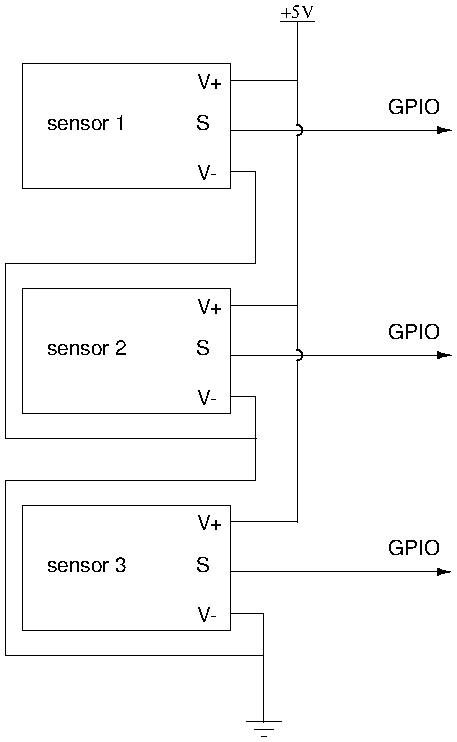
\includegraphics[scale=0.5]{circuitSensor.png}
\end{figure}


DESCRIZIONE DEI SENSORI CON FOTO

\subsection{Relè}

Poichè sarà necessario pilotare anche luci di abitazioni, gli slave non possono essere in grado di erogare abbastanza corrente per queste. Per risolvere questo problema, è necessario utilizzare un componente hardware chiamato Relè. Questo oggetto consiste in un avvolgimento di rame e una lamina di rame che funge da switch di canale; appena l'avvolgimento viene eccitato con la corrente, genera un campo magnetico che sposta la lamina di rame in modo da deviare la corrente da un canale all'altro. Anche la bobina di rame però necessita di molta corrente per generare un campo magnetico; è presente quindi un relè allo stato solido che riceve in input sia la corrente necessaria alla bobina per generare il campo magnetico sia la corrente dello slave per pilotare via software le luci; in output invierà la corrente necessaria per il relé solo quando lo slave invia il segnale.

Questo oggetto può quindi essere utilizzato come interruttore automatico pilotato dal processore. È stata utilizzata una scheda per pilotare 8 relè tramite le gpio di uno slave, in modo da accendere o spegnere le luci a led a basso consumo.


FOTO SCHEDA

\subsection{Luci a led}

PORTARE LUCI

%%%%%%%%%%%%%%%%%%%%%%%%%%%%%%%%%%%%%%%%%%%%%%%%%%%%%%%%%%%%%%%%%%%%%%%%%%%%%%%%%%%%%%%%%%%%%%%%%%%%%%%%%%%%%%%%%%%%%%%%%%%%%%%%%%%%%%%%%
%%%%%%%%%%%%%%%%%%%%%%%%%%%%%%%%%%%%%%%%%%%%%%%%%%%%%%%%%%%%%%%%%%%%%%%%%%%%%%%%%%%%%%%%%%%%%%%%%%%%%%%%%%%%%%%%%%%%%%%%%%%%%%%%%%%%%%%%%
%%%%%%%%%%%%%%%%%%%%%%%%%%%%%%%%%%%%%%%%%%%%%%%%%%%%%%%%%%%%%%%%%%%%%%%%%%%%%%%%%%%%%%%%%%%%%%%%%%%%%%%%%%%%%%%%%%%%%%%%%%%%%%%%%%%%%%%%%
%%%%%%%%%%%%%%%%%%%%%%%%%%%%%%%%%%%%%%%%%%%%%%%%%%%%%%%%%%%%%%%%%%%%%%%%%%%%%%%%%%%%%%%%%%%%%%%%%%%%%%%%%%%%%%%%%%%%%%%%%%%%%%%%%%%%%%%%%


\chapter{Architettura Software}

La parte più interessante di questo preambolo al progetto realizzato è lo scheletro software su cui si basa tutta la progettazione. È facile pensare alla programmazione in un ambiente in cui il sistema operativo offre un ``\textit{hardware abstraction layer}'' che garantisce una facile programmazione. Nell'ambito però dei sistemi embedded, un HAL è pressochè assente, quindi la programmazione si complica in quanto bisogna ragionare sul funzionamento dell'architettura stessa.


\section{Dispositivo Master}

Per LPC1788 il problema principale era quello di gestire l'interfaccia grafica e l'invio di messaggi agli Slave. Per gestire facilmente ciò, è stato utilizzato un sistema preconfezionato che offre delle API utili alla gestione di periferiche e per la progettazione. 


\subsection{uEZ}
Questo sistema si chiama $\mu EZ$, chiamato così perché dovrebbe ``ispirare'' il designer di software embedded durante la progettazione e semplificarla. In realtà ci sono stati dei problemi di scrittura di queste API da parte degli sviluppatori che hanno fatto l'esatto opposto (sono comunque state corrette e successivamente verrà spiegato).

~

\begin{figure}[!h]
\centering
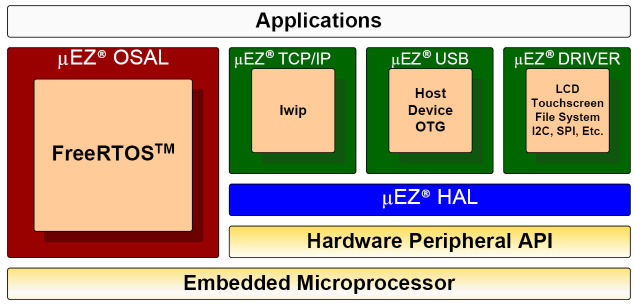
\includegraphics[scale=0.7]{uEZ.png}
\caption{architettura del sistema uEZ}\label{fig:1}
\end{figure}

Il sistema offre innanzitutto un HAL piuttosto potente, in quanto permette di trattare ad alto livello la configurazione di tutte le periferiche. Inoltre non è necessario definire il boot di sistema (cosa non banale per questi sistemi). Esiste un porting standard per ogni processore, se non è presente è possibile scriverlo facilmente. Il sistema deve essere compilato in due passaggi: il primo consiste nel compilare $\mu EZ$ per la propria architettura, ottenendo un file di libreria da linkare al proprio progetto, il secondo consiste nello sviluppare il proprio progetto basandosi su questo sistema. È possibile, al tempo di compilazione, decidere quali periferiche utilizzare prima di generare la libreria da linkare, ottimizzando per area il proprio software.

~

Ciò che ha portato allo sviluppo su questo sistema software è stato, oltre all'astrazione dell'hardware che facilita la programmazione, alla predisposizione da parte del sistema di usare risorse di rete come lo stack di rete lwIP e alla presenza di sistema operativo FreeRTOS, è stata la capacità di utilizzare una libreria grafica molto importante e potente per i sistemi embedded, la libreria \textbf{emWIN}.

\subsection{emWin}

Questa è una libreria grafica per sistemi embedded molto potente, basata su una grafica molto simile alle prime versioni di Windows (sia per l'estetica sia per la gestione ottimale delle risorse grafiche). Essa offre un HAL ad alto livello molto semplice da utilizzare, con cui è possibile progettare interfacce con oggetti grafici ben noti (bottoni, input text, ecc...) senza dover interfacciarsi direttamente con l'oggetto hardware. Può sembrare una soluzione poco ottimale, visto che tutti gli elementi ad ``alto livello'' nella progettazione di sistemi embedded può essere reputata poco efficiente in ambito di risorse e computazione, in realtà è stata progettata in maniera talmente sofisticata che risulta ancora più efficiente della scrittura ``a mano'' delle stesse librerie.

La gestione dell'interfaccia tramite questa libreria ha un'implementazione molto semplice:

\begin{enumerate}[noitemsep,topsep=18pt,parsep=10pt,partopsep=0pt]
\item si descrive l'interfaccia implementandola personalmente o tramite appositi programmi di generazione di codice (GUIBuilder incluso nel pacchetto emWin);
\item si associa al codice corrente l'intefaccia appena creata ricordandosi di usare il comando \\\lstinline!ExecDialogBox()! (vedere manuale emWin);
\item si associa ai widget creati il codice che viene eseguito in base agli eventi generati.

\end{enumerate}

Particolare interesse deve essere prestato al metodo con cui si può interagire con i widget: per modificare o eseguire azioni generiche sul widget, è necessario farsi restituire un puntatore specifico e lavorare su di esso. Un esempio di codice:

\begin{lstlisting}

#define ID_WIDGET ID_GUI + 0x00

...

EMWIN_WIDGET_TYPE my_widget;

...

WM_HWIN hItem = WM_GetDialogItem(pMsg->hWin, ID_WIDGET);
my_widget = my_value; 

\end{lstlisting}

~

Il porting che è stato fatto di questa libreria per questo processore dipende dalla board di sviluppo che si vuole considerare (soprattutto per il nostro LCD TouchScreen), nel nostro caso dipende in maniera esclusiva da $\mu EZ$. Infatti per questioni di modularità, emWin si appoggia alle API di $\mu EZ$, in modo da sfruttarle senza interfacciarsi direttamente con l'hardware sottostante , essendo già state ottimizzate le API di $\mu EZ$ (quindi emWin nel nostro caso non può funzionare senza di $\mu EZ$).
 
\section{Dispositivi Slave}

Questi dispositivi non hanno una parte software che funge da scheletro per l'applicazione, essenzialmente per due motivi:

\begin{itemize}[noitemsep,topsep=18pt,parsep=10pt,partopsep=0pt]

\item le architetture sono troppo semplici, non è necessario interfacciarsi con l'hardware tramite API visto che i comandi che devono eseguire sono diretti alle diverse periferiche;
\item non è presente molta memoria e non è garantita molta capacità di calcolo, quindi sarebbe svantaggioso utilizzare qualcosa di più ``astratto'' (e quindi inefficiente) per gestire le operazioni.

\end{itemize}

L'unica eccezione di questo argomento è l'utilizzo, per il dispositivo ARM, di un sistema operativo. Per il dispositivo PIC non è stato possibile inserire il sistema operativo, in quanto non è presente abbastanza memoria e il sistema di calcolo è troppo semplice.

\subsection{FreeRTOS}

Il sistema operativo utilizzato sul dispositivo di tipo ARM Cortex-M3 si chiama FreeRTOS. 

È un sistema operativo di tipo Real Time, ossia  il sistema deve essere ``prevedibile'' o piuttosto ``determinista'', nel senso che nel sistema si deve conoscere il tempismo reale (nei migliori o peggiori dei casi) di un determinato processo o elaborazione. In pratica un sistema real-time deve garantire che una elaborazione (o task) termini entro un dato vincolo temporale o scadenza (detta in gergo deadline). Per garantire questo è richiesto che la schedulazione delle operazioni sia fattibile. Il concetto di fattibilità di schedulazione è alla base della teoria dei sistemi real-time ed è quello che ci permette di dire se un insieme di task sia eseguibile o meno in funzione dei vincoli temporali dati.

Il sistema operativo non è stato utilizzato per utilizzare una HAL per programmare, ma per creare dei task separati per gestire la parte di protocollo e la parte di applicazione, in quanto continui polling sui sensori possono disturbare l'invio della risposta al dispositivo Master.



%%%%%%%%%%%%%%%%%%%%%%%%%%%%%%%%%%%%%%%%%%%%%%%%%%%%%%%%%%%%%%%%%%%%%%%%%%%%%%%%%%%%%%%%%%%%%%%%%%%%%%%%%%%%%%%%%%%%%%%%%%%%%%%%%%%%%%%%%
%%%%%%%%%%%%%%%%%%%%%%%%%%%%%%%%%%%%%%%%%%%%%%%%%%%%%%%%%%%%%%%%%%%%%%%%%%%%%%%%%%%%%%%%%%%%%%%%%%%%%%%%%%%%%%%%%%%%%%%%%%%%%%%%%%%%%%%%%
%%%%%%%%%%%%%%%%%%%%%%%%%%%%%%%%%%%%%%%%%%%%%%%%%%%%%%%%%%%%%%%%%%%%%%%%%%%%%%%%%%%%%%%%%%%%%%%%%%%%%%%%%%%%%%%%%%%%%%%%%%%%%%%%%%%%%%%%%
%%%%%%%%%%%%%%%%%%%%%%%%%%%%%%%%%%%%%%%%%%%%%%%%%%%%%%%%%%%%%%%%%%%%%%%%%%%%%%%%%%%%%%%%%%%%%%%%%%%%%%%%%%%%%%%%%%%%%%%%%%%%%%%%%%%%%%%%%

\chapter{Modello di sistema}

Di seguito si riporta il modello del sistema secondo lo standard ingegneristico, ossia presentando:
\begin{itemize}[noitemsep,topsep=23pt,parsep=23pt,partopsep=0pt]

\item\textit{``Use Case Diagram''}, ossia la presentazione ad alto livello dei diversi attori del sistema (nel nostro caso gli attori sono: l'utente, il dispositivo Master e il dispositivo Slave), in modo da rendere chiari i ruoli degli attori e le loro azioni all'interno dello scenario;
\item\textit{``Sequence Diagram''}, ossia la presentazione ad alto livello dello scambio di ``messaggi'' tra i diversi attori e dispositivi del sistema (vengono identificate le interazioni nel sistema come messaggi).

\end{itemize}

\newpage

\section{Use Case Diagram}

Con questo tipo di diagramma, viene presentata una tabella per ogni attore, ciascuna contenente nell'intestazione il nome dell'attore considerato e all'interno le rispettive azioni. Ogni attore coinvolto nel sistema ha delle precondizioni da rispettare affinchè tutte le operazioni vadano a buon fine e una postcondizione. Vengono presentate infine le azioni sotto forma di algoritmo o insieme di attività da svolgere per eseguire un task.

L'attore principale, cioè l'utente, ha tre tipi di attività, ossia la scelta del task da far eseguire al sistema, l'avvio di esecuzione di tale task (premendo l'opportuno tasto nell'interfaccia) e l'osservazione dei valori che vengono mostrati nella GUI.

L'altro attore è il dispositivo Master, che ha il compito di mostrare ed aggiornare l'interfaccia grafica e di interrogare il dispositivo Slave in base alla scelta dell'utente. Questo attore ha quindi queste attività: mostrare l'interfaccia grafica, avviare i task scelti dall'utente e inviare i messaggi ai dispositivi Slave.

Gli ultimi attori da considerare sono i dispositivi Slave, che hanno il compito di eseguire polling sui sensori a loro associati e di rispondere alle richieste Modbus del dispositivo Master. Le loro attività quindi sono: controllo sensori e ricezione e risposta di messaggi Modbus.

~

~

\begin{usecase}
  \addheading{Attore}{Utente} 
  \addrow{Precondizione}{Il sistema è avviato e mostra la GUI a seguito del logo $\mu EZ$, tutti i tasti sono selezionabili e tutti i dispositivi sono avviati. L'utente è munito di penna specifica per interfacciarsi col dispositivo TouchScreen.}
  \addrow{Postcondizione}{La scelta dell'utente è stata soddisfatta}
  \addmulrow{Scelta task}	{\item interfaccia gestione LED
                             	\item interfaccia monitoraggio sensori
				\item interfaccia di debug}

  \addmulrow{Esecuzione task}	{\item accendere o spegnere luci
                             	\item controllo sensori
				\item attività di debug}

  \addmulrow{Osserva valori}	{\item valutazione valori mostrati dalla GUI}

\end{usecase}

\begin{usecase}

  \addheading{Attore}{Master} 
  \addrow{Precondizione}{Il sistema è avviato.}
  \addrow{Postcondizione}{L'utente esegue correttamente scelte.}
  \addmulrow{Mostra GUI}	{\item mostra schermata principale}

  \addmulrow{Avvia task}	{\item ottieni scelta dall'utente}

  \addmulrow{Invia messaggi}	{\item messaggi di tipo read
				\item messaggi di tipo write}
  

\end{usecase}


\begin{usecase}

  \addheading{Attore}{Slave} 
  \addrow{Precondizione}{Il sistema è avviato, i sensori rispondono e si ricevono correttamente messaggi Modbus.}
  \addrow{Postcondizione}{Si risponde al messaggio Modbus.}
	\addmulrow{Controllo}	{\item esegue polling sui sensori
				\item aggiorna il valore dei registri col valore ottenuto dai sensori}
  \addmulrow{Ricezione}		{\item riceve messaggi Modbus
				\item invia o setta i registri richiesti }

\end{usecase}


\newpage

\section{Sequence Diagram}

Questo diagramma rappresenta una generica interazione tra utente e sistema. Ad ogni scelta dell'utente, visualizzabile come un messaggio (ovviamente non testuale) inviato dall'utente al dispositivo Master, viene trasformata in messaggio Modbus da inviare al corrispondente dispositivo Slave. Il dispositivo Slave, prima di essere interrogato via Modbus, continua ad eseguire polling sui sensori a lui collegati, per tenersi aggiornato sul loro valore. Al momento della richiesta Modbus, il disposivo Slave termina momentaneamente di eseguire polling sui sensori e invia l'ultimo valore acquisito da questi al dispositivo Master. Quest'ultimo, appena riceve i valori, aggiorna l'interfaccia grafica e mostra all'utente il risultato dell'interrogazione. Fatto ciò, il dispositivo Master rimane in attesa di ordini dall'utente, mentre il dispositivo Slave continua a fare polling sui sensori a lui collegati.

~

\begin{figure}[!hb]
  \centering
  \begin{sequencediagram}

    \newthread{ut}{:Utente}	%rettangolo sempre attivo
    \newinst[2.5]{ms}{:Master}		%solo tratteggiato
    \newinst[2.5]{sl}{:Slave}

        \begin{callself}{sl}{PollSensori()}{}
        \end{callself}
        \begin{callself}{sl}{PollSensori()}{}
        \end{callself}
        \begin{callself}{sl}{PollSensori()}{}
        \end{callself}
    
      	\begin{call}{ut}{EseguiScelta()}{ms}{}

		\begin{call}{ms}{inviaRichiestaModbus()}{sl}{}
		\end{call}

		\begin{callself}{ms}{aggiornaGUI()}{}
		\end{callself}



      	\end{call}

		\begin{callself}{sl}{PollSensori()}{}
		\end{callself}
		\begin{callself}{sl}{PollSensori()}{}
		\end{callself}
		\begin{callself}{sl}{PollSensori()}{}
		\end{callself}


  \end{sequencediagram}
  \caption{Esempio di attività generica con il sistema.}
\end{figure}



%%%%%%%%%%%%%%%%%%%%%%%%%%%%%%%%%%%%%%%%%%%%%%%%%%%%%%%%%%%%%%%%%%%%%%%%%%%%%%%%%%%%%%%%%%%%%%%%%%%%%%%%%%%%%%%%%%%%%%%%%%%%%%%%%%%%%%%%%
%%%%%%%%%%%%%%%%%%%%%%%%%%%%%%%%%%%%%%%%%%%%%%%%%%%%%%%%%%%%%%%%%%%%%%%%%%%%%%%%%%%%%%%%%%%%%%%%%%%%%%%%%%%%%%%%%%%%%%%%%%%%%%%%%%%%%%%%%
%%%%%%%%%%%%%%%%%%%%%%%%%%%%%%%%%%%%%%%%%%%%%%%%%%%%%%%%%%%%%%%%%%%%%%%%%%%%%%%%%%%%%%%%%%%%%%%%%%%%%%%%%%%%%%%%%%%%%%%%%%%%%%%%%%%%%%%%%
%%%%%%%%%%%%%%%%%%%%%%%%%%%%%%%%%%%%%%%%%%%%%%%%%%%%%%%%%%%%%%%%%%%%%%%%%%%%%%%%%%%%%%%%%%%%%%%%%%%%%%%%%%%%%%%%%%%%%%%%%%%%%%%%%%%%%%%%%



\chapter{Implementazione del sistema}


A seguito di tutte le considerazioni sul modello di sistema e sulla tecnologia utilizzata, è stato deciso di utilizzare un protocollo di comunicazione industriale standard chiamato \textit{Modbus}, che sfrutta la comunicazione seriale, un'interfaccia grafica basata su \textit{emWin} e uno strato applicativo che verrà discusso in questa sezione. 

\section{Protocollo Modbus}


Modbus è un protocollo semplice di tipo Master-Slave, cioè esiste un dispositivo centrale che invia una richiesta e i diversi slave soddisfano la richiesta dando una risposta al Master. Il dispositivo Master è sempre pronto ad inviare una richiesta, mentre gli Slave rimangono sempre in ascolto e non inviano alcun tipo di messaggio se non vengono interpellati dal Master.

~

Questo protocollo è stato progettato in modo da far comunicare un Master con un massimo di 256 Slave, inviando un messaggio in cui si specifica l'indirizzo del destinatario Slave e il tipo di richiesta. Quando uno Slave riceve un messaggio, controlla se gli appartiene tramite l'indirizzo del messaggio, altrimenti lo scarta; questo deve avvenire poichè la comunicazione seriale non necessita di apparecchiature che indirizzano il messaggio al giusto destinatario, ma la comunicazione è garantita da una rete di ``fili'' che collegano i diversi dispositivi.

\subsection{Tipi di messaggi}

Il messaggio tipico del protocollo è formato da questi campi:

~

~

\begin{tabular}{|c  c  c|}
\hline
\multicolumn{1}{|c|}{\textbf {campo}} & \multicolumn{1}{c}{\textbf {byte}} & \multicolumn{1}{|c|}{\textbf {descrizione}} \\
\hline
Indirizzo	&	1	&	l'indirizzo del dispositivo con cui il master ha stabilito la transazione\\

Funzione	&	1	&	il codice della funzione che deve essere o è stata eseguita \\

Dati		&	2 $\cdot$ n\_dati	&	i dati che devono essere scambiati tra i due dispositivi in base alla funzione scelta \\

CRC		&	2			&	il controllo d'errore composto secondo l'algoritmo CRC16 \\

\hline
\end{tabular}

~

~

Se un dispositivo individua un errore nel messaggio ricevuto (di formato, di parità o nel CRC16) il messaggio viene considerato non valido e viene notificato al Master (o scartato); se uno slave quindi rileva un errore nel messaggio, non eseguirà l'azione e non risponderà alla domanda, così come se ricevesse un messaggio con l'indirizzo non corrispondente al suo.


\subsection{Registri}

Il protocollo Modbus permette la comunicazione tra master e slave tramite diversi tipi di variabili chiamate ''registri``. In base al tipo di registro, sono permesse diverse operazioni:

\begin{itemize}[noitemsep,topsep=15pt,parsep=10pt,partopsep=0pt]

\item i registri di \textbf{``Input''} rappresentano dei booleani (registri a bit singolo) che possono essere solo letti, quindi in questi può essere eseguita una funzione di tipo read;
\item i registri di \textbf{``Input Discreti''} hanno lo stesso funzionamento, in generale il master può solo leggere i registri di questo tipo;
\item i registri di \textbf{``Holding''} rappresentano una word a 16 bit che può essere sia letta sia scritta;
\item i registri di \textbf{``Coil''} rappresentano un booleano che può essere sia letto che scritto dal Master;

\end{itemize}

Ogni registro può essere quindi associato ad una variabile di stessa grandezza o che rappresenta una grandezza simile (facendo un opportuno cast). Il motivo per cui vengono identificate queste variabili come registri deriva dal fatto che questo protocollo veniva utilizzato in un sistema in cui erano effettivamente presenti dei registri fisici associati a componenti hardware. In particolare i registri di Coil erano associati a dei Relè (infatti Coil significa ''avvolgimento``) e per questo vengono rappresentati con un booleano (1 e 0 rappresentano bene la situazione acceso-spento).

\subsection{Tipi di richiesta}

Modbus ha diversi tipi di richiesta, ognuna riguardante un registro specifico:

~

~

\begin{tabular}{|c  c  c|}
\hline
\multicolumn{1}{|c|}{\textbf {Numero funzione}} & \multicolumn{1}{c}{\textbf {Nome funzione}} & \multicolumn{1}{|c|}{\textbf {Registro associato}} \\
\hline
01 & Read Coil Status		&	Coil		\\
02 & Read Input Status		&	Input		\\
03 & Read Holding Registers	&	Holding		\\
04 & Read Input registers	&	Input Discreto	\\
05 & Force Single Coil		&	Coil		\\
06 & Prese Single register	&	Holding		\\
15 & Force multiple Coils	&	Coil		\\
16 & Preset Multiple Registers	&	Holding		\\
\hline
\end{tabular}

~

~

Viene riportata di seguito la descrizione dettagliata delle funzioni più utilizzate:

\begin{itemize}[noitemsep,topsep=15pt,parsep=10pt,partopsep=0pt]
\item \textbf{Read Coil Status (01)}: permette di richiedere lo stato ON o OFF di variabili logiche binarie (registri
output R/W).
La modalità broadcast non è permessa.
\item \textbf{Read Input Status (02)}: è operativamente identica alla precedente ma riguarda i registri input.
\item \textbf{Read Output Registers (03)}: permette di richiedere il valore di registri a 16 bit (word) contenenti variabili numeriche (registri output R/W). La modalità broadcast non è permessa.
\item \textbf{Read Input Registers (04)}: è operativamente identica alla precedente ma riguarda i registri Input.
\item \textbf{Force Single Coil (05)}: permette di forzare lo stato di una singola variabile binaria ON o OFF. La modalità broadcast è permessa.
\item \textbf{Preset Single Register (06)}: permette di impostare il valore di un singolo registro a 16 bit. La modalità broadcast è permessa.
\item \textbf{Force Multiple Coils (15)}: permette di forzare lo stato di ciascuna variabile binaria in un blocco consecutivo. La modalità broadcast è permessa.
\item \textbf{Preset Multiple Registers (16)}: permette di impostare il valore di un blocco consecutivo di registri a 16 bit. La modalità broadcast è permessa.

\end{itemize}

\subsection{CRC16}

Gli ultimi due caratteri del messaggio contengono il codice di ridondanza ciclica (Cyclic Redundancy Check) calcolato secondo l'algoritmo CRC16.

~

Per il calcolo di questi due caratteri il messaggio (indirizzo, codice funzione e dati scartando i bit di start, stop e l'eventuale parità) viene considerato come un unico numero binario ``continuo'' di cui il bit più significativo (MSB) viene trasmesso prima. La procedura passo-passo per il calcolo del CRC16 è la seguente:

\begin{enumerate}[noitemsep,topsep=15pt,parsep=10pt,partopsep=0pt]

\item Caricare un registro a 16 bit con FFFFh (tutti i bit a 1).
\item Fare l'OR esclusivo del primo carattere con il byte superiore del registro , porre il risultato nel registro.
\item Spostare il registro a destra di un bit.
\item Se il bit uscito a destra dal registro (flag) è un 1, fare l'OR esclusivo del polinomio generatore 1010000000000001 con il registro.
\item Ripetere per 8 volte i passi 3 e 4.
\item Fare l'OR esclusivo del carattere successivo con il byte superiore del registro, porre il risultato nel registro.
\item Ripetere i passi da 3 a 6 per tutti i caratteri del messaggio.
\item Il contenuto del registro a 16 bit è il codice di ridondanza CRC che deve essere aggiunto al messaggio

\end{enumerate}

Questa parte del messaggio è particolarmente importante perché garantisce la correttezza del messaggio; in un sistema industriale, quindi disturbato, è possibile che un messaggio su seriale possa essere afflitto da disturbi, quindi è necessario garantire la sicurezza della richiesta. Comandare un dispositivo con un messaggio sbagliato corrisponde a fare danni al sistema o a ciò che lo circonda. In un contesto casalingo, potrebbe non crea molti danni, però può creare disagio; ad esempio, se piove e l'utente vuole chiudere le finestre, se il messaggio risulta corrotto potrebbe essere interpretato come ``aprire le finestre'' e ciò crea problemi.

\subsection{Sincronizzazione}
La sincronizzazione del messaggio tra trasmettitore e ricevitore viene ottenuta interponendo una pausa tra i messaggi pari ad almeno 3.5 volte il tempo di un carattere. Se il dispositivo ricevente non riceve per un tempo di 3,5 caratteri, ritiene completato il messaggio precedente e considera che il successivo byte ricevuto sarà il primo di un nuovo messaggio e quindi un indirizzo.


\section{Implementazione del protocollo Modbus}

Per implementare questo protocollo, sono state prese due vie alternative, rispettivamente per il dispositivo Master e per i dispositivi Slave:

\begin{itemize}[noitemsep,topsep=15pt,parsep=10pt,partopsep=0pt]

\item Master: è stato implementato il protocollo basandosi sulla descrizione dello standard;
\item Slave: è stato eseguito il porting di una libreria chiamata FreeModbus e la creazione di una libreria ridotta MiniModbus.

\end{itemize}

Di seguito verranno descritte le implementazioni nel dettaglio.

\subsection{Master}

L'implementazione del software del dispositivo Master è molto più semplice dello Slave e la procedura per la programmazione non presenta particolari problemi.

~

Per prima cosa, bisogna aggiungere una struttura dati che consente di manipolare facilmente i messaggi Modbus. La struttura presente nel progetto è la seguente:

\begin{lstlisting}[showlines=false]
typedef struct
   {
      int8_t address; //indirizzo del ricevente
      int8_t len;    //numero di byte del messaggio
      function func; //funzione richiesta del messaggio
      exception error;  //eccezione riscontrata nel messaggio
      int8_t data[MODBUS_SERIAL_RX_BUFFER_SIZE]; //sezione dati del messaggio
      int16_t data_converted[125];  //dati omogenei convertiti
   }_modbus_rx;
\end{lstlisting}

In questo modo, si semplifica notevolmente il lavoro di interpretazione del messaggio: ogni carattere potrà popolare i campi di questa struttura, essendo anche ottimizzati rispetto alla grandezza dei byte. 

Bisogna notare che il campo CRC non è presente, in quanto l'elaborazione di questo non è utilizzata all'esterno del protocollo e deve essere calcolato real time durante la ricezione del messaggio (quindi non serve memorizzarlo).

Bisogna notare inoltre che esiste una sezione \lstinline!data[]! diversa da \lstinline!data_converted[]!, poiché i dati arrivano a coppie di byte (memorizzati in \lstinline!data[]!), in modo da rappresentare non un \lstinline!char! ma una \lstinline!word!; in questo modo si può rappresentare un numero molto più grande, però deve essere convertito shiftando i bit dei due singoli \lstinline!char! in una singola \lstinline!word!. Questo spiega perché vengono rappresentate da variabili di tipo diverso, ossia un \lstinline!int8_t! per il \lstinline!char! e \lstinline!int16_t! per la \lstinline!word!.

~

~

Successivamente bisogna attivare e dirigere nel dispositivo la seriale e il timer interno; in questo modo si implementa la ricezione e invio dei messaggi e la sincronizzazione dei dispositivi. Dal momento che la sincronizzazione corrisponde a ``contare'' il tempo tra un carattere e l'altro (quando il Master riceve la risposta), basta attivare un timer appena si riceve il primo carattere di risposta e comportarsi come segue:

\begin{enumerate}[noitemsep,topsep=15pt,parsep=6pt,partopsep=0pt]

\item rimango in ascolto per leggere un carattere e contemporaneamente conto;
\item ho finito di contare?
	\begin{itemize}
	\item SI, allora ho terminato la lettura del messaggio;
	\item NO, allora continuo ad ascoltare;
	\end{itemize}
\item ho ricevuto un carattere?
	\begin{itemize}
	\item SI, allora resetto il contatore quindi ricomincio a contare da 0, poi torno al punto 1;
	\item NO, allora torno al punto 1;
	\end{itemize}

\end{enumerate}

Nel codice, è stata usata una variabile chiamata \lstinline!modbus_serial_wait! che rappresenta il tempo contato secondo il delay gestito dalla API di $\mu EZ$ \lstinline!void delay_us(int us)!; finchè non ci sono caratteri disponibili, il valore di questa variabile viene decrementato ogni millisecondo finché non vale zero (indica il tempo scaduto).

Il codice che si occupa di questo è rappresentato dalla funzione sotto trascritta, presente nel file \textit{modbus\_function.c}:

\begin{lstlisting}[showlines=true,firstline=1, firstnumber=110]
void MODBUS_SERIAL_WAIT_FOR_RESPONSE()
{
        modbus_serial_state=MODBUS_GETADDY;
        modbus_serial_new = TRUE;

        while(--modbus_serial_wait >= 0)
          //se non ci sono caratteri disponibili, aspetto o vado in timeout
          if(!modbus_kbhit())
            delay_us(1);
          else
          //resetto il timer per 30 ms e mi preparo per aspettare di nuovo
            modbus_serial_wait=30;

        //se non ho letto nulla
        if(frame_received == FALSE)
           //errore!
           modbus_rx.error=TIMEOUT;

        else
           modbus_rx.error = 0;


        modbus_serial_wait = MODBUS_SERIAL_TIMEOUT;
        modbus_serial_new = TRUE;
        frame_received = FALSE;

}
\end{lstlisting}

Per quanto riguarda la seriale, visto che il sistema utilizzato è molto semplice (quindi senza gestione ad alto livello degli eventi del sistema), l'unico modo per non sprecare cicli di clock per il polling su seriale è stato quello di utilizzare gli interrupt. È stato quindi implementato un sistema di interrupt che si potesse adattare al protocollo Modbus: ad ogni carattere ricevuto si attiva la funzione \lstinline!uart_rx_interrupt()!,  in base al contatore globale dei caratteri (la variabile \lstinline!modbus_serial_state!) si gestisce in maniera automatica l'interpretazione dei singoli caratteri inserendoli nel campo giusto della struttura dati, incrementando, dopo aver acquisito un nuovo carattere, il valore di questa variabile. Di fatto questa rappresenta la ``posizione'' che ha il carattere appena ricevuto all'interno della struttura dati.
In particolare questa variabile acquisisce questa forma:

\begin{lstlisting}[showlines=false]

enum {
	MODBUS_GETADDY=0, 
	MODBUS_GETFUNC=1, 
	MODBUS_GETDATA=2 
			} modbus_serial_state;

\end{lstlisting}

questa enumerazione rappresenta con il primo campo la parte di indirizzo del messaggio, la seconda indica la funzione, la terza la sezione dati. In questo modo è molto più semplice (ed ottimizzato) gestire l'inserimento dei valori nella struttura.
\newpage
Il codice associato a questa procedura si trova nel file \textit{modbus\_function.c}:

\begin{lstlisting}[showlines=true, firstnumber=202]
void uart_rx_interrupt(void)
{

   char c;

   c = UART_ReceiveByte(_LPC_UART);


      if(modbus_serial_state == MODBUS_GETADDY)
      {
         modbus_serial_crc.d = 0xFFFF;
         modbus_rx.address = c;
         modbus_serial_state++;
         modbus_rx.len = 0;
         modbus_rx.error=0;
      }
      else if(modbus_serial_state == MODBUS_GETFUNC)
      {
         modbus_rx.func = c;
         modbus_serial_state++;
      }
      else if(modbus_serial_state == MODBUS_GETDATA)
      {
         if (modbus_rx.len>=MODBUS_SERIAL_RX_BUFFER_SIZE) 
		modbus_rx.len=MODBUS_SERIAL_RX_BUFFER_SIZE-1;

         modbus_rx.data[modbus_rx.len]=c;
         modbus_rx.len++;
      }

      Message[indix++] = c;

  modbus_serial_new = FALSE;
  frame_received = TRUE;

}
\end{lstlisting}

\subsection{Slave}


L'implementazione del protocollo di tipo Slave è molto diversa e risulterebbe molto più complessa di quella di un generico Master.

\subsubsection{FreeModbus}

Esiste una libreria embedded ``portabile'' (dal punto di vista implementativo) chiamata \textbf{FreeModbus}, che propone uno stack Modbus completo a patto che si scriva il porting delle funzioni che si interfacciano con il nostro hardware. Queste funzioni riguardano la seriale e il timer, utilizzate per lo stesso motivo del Master, e si trovano nei rispettivi file di porting:

\begin{itemize}[noitemsep,topsep=15pt,parsep=6pt,partopsep=0pt]

\item \textit{portserial.c}
\item \textit{porttimer.c}

\end{itemize}


Nel file \textit{portserial.c} è necessario modificare le funzioni di interrupt, di come si ricevono i caratteri da seriale e come si inviano. Nel file \textit{porttimer.c} si modifica invece l'interrupt del timer e la modalità di attivazione e setting. In entrambi i casi, bisogna scrivere la funzione di inizializzazione della corretta periferica. È importante sapere che bisogna cambiare il contenuto delle funzioni, ma non il nome, perché le altre funzioni dipendono dai nomi già scritti.

In particolare per \textit{portserial.c} bisogna implementare queste funzioni:

\begin{lstlisting}
//abilitazione dei canali Rx e Tx
void vMBPortSerialEnable( BOOL xRxEnable, BOOL xTxEnable )
{
	...
}

//chiusura porta seriale
void vMBPortClose( void )
{
	...
}

//inizializzazione della porta seriale
BOOL xMBPortSerialInit( UCHAR ucPORT, 
			ULONG ulBaudRate, 
			UCHAR ucDataBits, 
			eMBParity eParity )
{
	...
}

//invio di un carattere
BOOL xMBPortSerialPutByte( CHAR ucByte )
{
	...
}

//ricezione di un carattere
BOOL xMBPortSerialGetByte( CHAR * pucByte )
{
	...
}

//interrupt della seriale
BOOL UART_IRQHandler( void )
{
	...

	/* Receive Data Available */
	prvvUARTRxISR(  );

	...
}
\end{lstlisting}

~

mentre per \textit{porttimer.c} bisogna implementare queste funzioni:

\begin{lstlisting}
//inizializzazione del timer
BOOL xMBPortTimersInit( USHORT usTim1Timerout50us )
{
	...
}

//abilitazione start del timer
void vMBPortTimersEnable(  )
{
	...
}

//stop del timer e reset
void vMBPortTimersDisable(  )
{
	...
}

//interrupt del timer
void TIMER0_IRQHandler(void)
{
	( void )pxMBPortCBTimerExpired(  );
	...
}


\end{lstlisting}


Una volta implementate queste funzioni, è necessario creare i registri nel main e le relative funzioni per interfacciarsi con essi. Dei registri bisogna, prima di dichiararli sotto forma di variabili, scrivere il loro ``indirizzo fisico'', cioè l'indirizzo da cui si parte a contarli (è arbitrario) e quanti se ne vogliono creare. Tutto questo è da fare tramite delle macro, in modo da poter verificare tramite protocollo le corrette richieste Modbus, per poter generare un errore da protocollo (NON da software, perché significherebbe andare a leggere o a scrivere in una zona di memoria non consona e quindi si genererebbe un grave errore o uno stallo di sistema). Un esempio:

\begin{lstlisting}

//indirizzo dei registri di input
#define REG_INPUT_START 1000
//quantita' di registri di input	
#define REG_INPUT_NREGS 4	

//indirizzo dei registri di holding
#define REG_HOLDING_START 2000
//quantita' di registri di holding	
#define REG_HOLDING_NREGS 130	

//assegnamento alla variabile nota alle API
static USHORT   usRegHoldingStart = REG_HOLDING_START;
//dichiarazione dei registri di holding	
static USHORT   usRegHoldingBuf[REG_HOLDING_NREGS];	

//assegnamento alla variabile nota alle API
static USHORT   usRegInputStart = REG_INPUT_START;
//dichiarazione dei registri di input	
static USHORT   usRegInputBuf[REG_INPUT_NREGS];		

\end{lstlisting}


\subsubsection{MiniModbus}

Poichè l'architettura target non sempre offre grande disponibilità di memoria e di stack, è necessario utilizzare una libreria più ottimizzata e performante in modo che possa offrire il protocollo Modbus anche nelle architetture più semplici. Per questo motivo è stata implementata una libreria ``portabile'' (dal punto di vista implementativo) che è stata chiamata MiniModbus. Questa libreria offre le stesse potenzialità della libreria FreeModbus, però risulta più performante per le architetture meno potenti (come i microcontrollori e i microprocessori di fascia bassa).

L'architettura target in questo caso è stata il PIC16F77 che, come è stato descritto, ha $2^8$ spazi di indirizzamento di memoria. FreeModbus necessita di $2^{16}$ spazi di indirizzamento di memoria e quindi risulta troppo grande per il PIC. Inoltre questa architettura permette $2^6$ byte di locazioni di memoria contigua, mentre Modbus vuole una lunghezza di messaggi uguale a 256 byte, quindi $2^8$ byte, quindi la lunghezza del messaggio è stata ridotta a 64 byte. 

~

Per eseguire il porting di questa libreria è necessario modificare il file \textit{modbus\_port.c} riscrivendo il contenuto di queste funzioni (sostituendo al posto dei puntini la rispettiva implementazione):

\begin{lstlisting}

//implementazione del delay per millisecondi
void delay_us(uint32_t delayInMs)
{
    ...
}

//abilitazione del timer
void TimersEnable(  )
{
    ...
}

//disabilitazione del timer
void TimersDisable(  )
{
    ...
}

//attiva ricezione seriale
void RCV_ON(void)
{
    ...
}

//disabilita ricezione seriale
void RCV_OFF(void)
{
    ...
}

//abilita il timeout (per il fine messaggio)
void modbus_enable_timeout(BOOL enable)
{
   if (enable) {

    ...

   }

   else
    ...

}

//scrive un carattere su seriale
void modbus_serial_putc(int8_t c)
{
	Message[indix] = c;
	indix++;

    ...

}

//interrupt generato dalla ricezione di un byte su seriale
void uart_rx_interrupt(void)
{
   char c = ... //ricezione del carattere dal canale seriale

   //nuovo carattere ricevuto
   modbus_serial_new = TRUE;

      if(modbus_serial_state == MODBUS_GETADDY)
      {
         modbus_serial_crc.d = 0xFFFF;
         modbus_rx.address = c;
         modbus_serial_state++;
         modbus_rx.len = 0;
         modbus_rx.error=0;
      }
      else if(modbus_serial_state == MODBUS_GETFUNC)
      {
         modbus_rx.func = c;
         modbus_serial_state++;
      }
      else if(modbus_serial_state == MODBUS_GETDATA)
      {
         if (modbus_rx.len>=MODBUS_SERIAL_RX_BUFFER_SIZE) 
		modbus_rx.len=MODBUS_SERIAL_RX_BUFFER_SIZE-1;

         modbus_rx.data[modbus_rx.len]=c;
         modbus_rx.len++;
      }

      Message[indix++] = c;

      modbus_enable_timeout(TRUE);

}

\end{lstlisting}

È importante sostituire solo dove ci sono i puntini le rispettive implementazioni delle funzioni. Una volta eseguito il porting di queste funzioni, si può prendere il codice presente e utilizzarlo per la propria architettura (file \textit{modbus.h, modbus.c, port.c, port.h, modbus\_port.h, modbus\_port.c, utils.c, utils.h}).


\section{Interfaccia grafica}

DA SCRIVERE

\subsection{Menù principale}
DA SCRIVERE
\subsection{Controllo Luci}
DA SCRIVERE
\subsection{Controllo Sensori}
DA SCRIVERE
\subsection{Schermata di Debug}
DA SCRIVERE

\section{Interazione con i componenti hardware}

È stato deciso di dividere la gestione delle componenti hardware come segue.

\subsection{Sensori}

I sensori vengono pilotati e controllati dal processore LPC1768, in quanto offre un'interfaccia semplice per la gestione di questi componenti, oltrechè offre più sicurezza di controllo di questi. Infatti, avendo un sistema operativo, si è in grado di gestire il controllo dei sensori su threads diverse, in modo che non si sprechino risorse e che quindi il processore non riesca a gestire la parte più importante di tutto il sistema, ossia la comunicazione.

~

Per questo motivo questo slave è in grado di interpretare messaggi sia di lettura/scrittura di registri di holding, sia di registri di coil. I registri di holding verranno utilizzati per memorizzare ed inviare i valori ottenuti dal sensore di temperatura e di umidità, mentre i registri di coil per i sensori di vibrazione, di luce, di distanza e di ostacolo.

\subsection{Relè e luci}

I relè, e quindi anche le luci a led, vengono pilotati tramite il microcontrollore PIC16F77, in quanto non è in grado di eseguire operazioni troppo onerose (controllare in polling dei sensori non darebbe la possibilità di comunicare via Modbus) e offre un'interfaccia semplice di invio segnali digitali ai relè. Quando verrà attivato il segnale da parte del PIC, i relè verranno percorsi da corrente, creando quindi il contatto necessario per far ricevere corrente alle luci.

~

Per questo, lo slave è in grado di interpretare solo messaggi di lettura/scrittura coil, poiché rappresentano bene il messaggio di on/off dei relè. Nell'architettura di origine di questo protocollo infatti i registri di coil venivano associati direttamente ai relè collegati al PLC. 


\section{Diagramma dei componenti}

Di seguito si riporta l'organizzazione di tutto il progetto

\subsection{Architettura Hardware}
DA SCRIVERE

\subsection{Architettura Software}
\begin{figure}[!h]
\centering
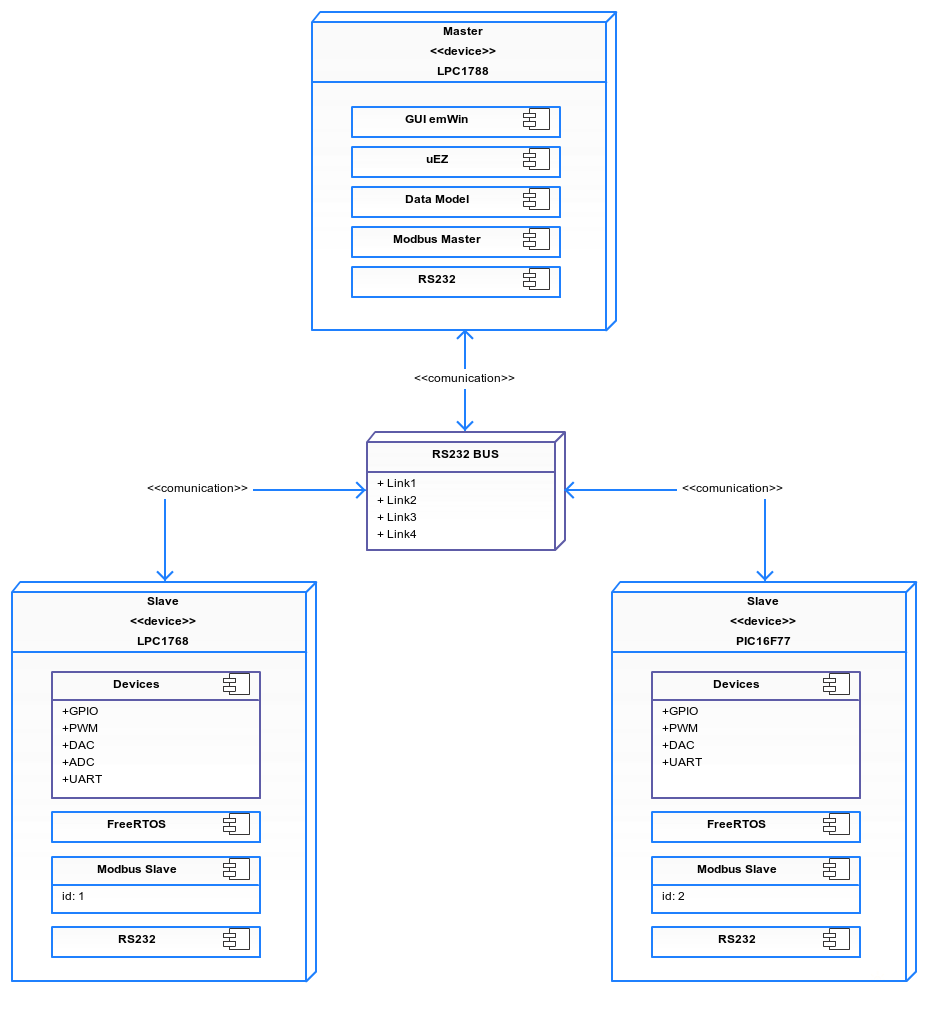
\includegraphics[scale=0.3]{deploy.png}
\caption{architettura del sistema}\label{fig:1}



\end{figure}


\chapter{Programmi utilizzati}

\section{LPC1788}


\section{LPC1768}


\section{PIC16F77}


\end{document}
\endinput
